\documentclass[a4paper,12pt]{report}
\usepackage[english]{babel}
\usepackage{graphicx}
\usepackage{placeins}
\usepackage{hyperref}

\title{TICCLops Documentation \\ \small version 0.0.1}
\author{Martin Reynaert \\ Induction of Linguistic Knowledge Research Group \\  Tilburg centre for Cognition and Communication \\Tilburg University }


\newenvironment{devnotes}
{\newpage
\begin{center}
    \begin{tabular}[h!]{|p{0.8\textwidth}|}
    \hline
    {\bf Development Notes}\\\hline}
{   \\\hline
    \end{tabular}
\end{center}}


\begin{document}

\maketitle
\tableofcontents

\chapter{Introduction} 


The spelling and OCR-error correction system Text-Induced Corpus Clean-up (TICCL) gradually developed by Martin Reynaert in prior projects at ILK is now TICCLops (TICCL online processing system), a fully operational web application and RESTful web service. This is thanks to the Computational Linguistics Application Mediator (CLAM), developed by Maarten van Gompel, also at ILK.

CLAM and TICCLops are the result of Call 1 in the CLARIN-NL programme, a Dutch initiative in the wider European CLARIN framework. The project TICCLops (CLARIN-NL/09-011) ran from February, 1st to July, 31st of 2010. The project was coordinated by Martin Reynaert. Maarten van Gompel was the scientific programmer. Martha van den Hoven, as student-assistant, did part of the work on the documentation.

\begin{devnotes}
TICCLops was designated the first step in the language technology tools workflow being developed within the CLARIN-NL project TTNWW. As a consequence, both TICCLops and to a larger extent CLAM are still under development. As such, this documentation is not definitive, but a work in progress.
\end{devnotes}

\chapter{Functional description of TICCL}

\section{Global description of TICCL}

TICCL (Text Induced Corpus Clean-up) is a system that is designed to search a corpus for all existing variants of (potentially) all words occurring in the corpus. This corpus can be one text, or several, in one or more directories, located on one or more machines. TICCL creates word frequency lists, listing for each word type how often the word occurs in the corpus. These frequencies of the normalized word forms are the sum of the frequencies of the actual surface forms found in the corpus.
TICCL is a system that is useful to detect typographical errors (misprints) and OCR errors (optical character recognition) in texts. When books or other texts are scanned from paper by a machine, that turns these scans into digital text-files, errors occur. For instance, the letter combination `in' can be read as `m', and so the word `regeering' is incorrectly read as `regeermg'. TICCL can be used to detect these errors and suggest a correct form.

TICCL's main goal is to output a list of focus words together with their variants, or correction candidates. A focus word is the word form that is found in the input corpus. What are considered to be variants depends on the maximum difference, which is an input parameter of TICCL. This maximum edit distance is measured in terms of Levenshtein distance. If there is a one-letter difference in a word pair, this counts as 1 edit cost. It does not matter if the one letter is an extra letter in the variant (insertion), a missing letter in the variant (deletion), or a different letter (substitution). If two letters should change places, this counts as an edit cost of 2 (transposition).

We give some examples in Table~\ref{Damerau}.

\begin{table}
%\begin{small}
\begin{center}
\caption{Edits\label{Damerau}}
\begin{tabular}{|l|l|l|c|}
\hline
Correct word & Variant & Name & Cost\\
\hline\hline
regering & regeering & insertion & 1\\
regering  & regerng	& deletion & 1\\
regering  & regeriug	& substitution & 1\\
regering  & regernig	& transposition & 2\\
regering  & regermg	& substitution + deletion & 1 + 1\\\hline
\end{tabular}
\end{center}
%\end{small}
\end{table}

If TICCL is run with a maximum edit distance of 1, the first three variants given in the example will be paired up with the correction candidate regering , the others won�t. The maximum possible edit distance that TICCL works with is 3. The bigger the edit distance used, the higher the number of false positives, meaning supposed variants of a focus word are retrieved, that are in reality not variants of the focus word, but different words. If the maximum edit distance is chosen too small, not all variants of a focus word are retrieved. A maximum edit distance of 2 usually gives the best results.

TICCL returns the number of types (distinct word forms) and tokens (total number of words in the corpus). Also the type/token ratio is returned. In a normal corpus, this ratio will be about 50\%. However, if there are many OCR-errors in the texts, the ratio can be much higher.

It is also possible to evaluate how well TICCL is doing. In order to do that, a so-called gold standard evaluation file is needed, which contains the text of the corpus. In this file are all misrecognised words in the OCR-ed version of the book, lined up with their correct or canonical form. Any variant of a focus word returned by TICCL, which is also in the gold standard, is counted as a true positive. Any variant returned by TICCL that is not in the gold standard, is a false positive. Any variant not returned by TICCL, but that exists in the gold standard, is a false negative. In this way of measuring how well TICCL performs no account is taken of the correct words in the OCR for which TICCL does not report anything. For more in depth information about spelling correction evaluation, please refer to \cite{Reynaert08c}.

%(TODO so what are the variants of a focus word that exist in the gs? For instance, regering vs. regeling, with edit distance 1? Because the gs does not contain any misspelled words, right?)

The user can influence the amount and type of words that TICCL tries to find variants for. It is possible to set criteria for word frequency and word length, so TICCL uses only words that match those criteria from the word frequency list it builds from the corpus.

%It is also possible for TICCL to output a list of processed files, together with a list of normalized word forms, with references to the files these word forms appear in. These lists can be the basis for correcting errors and adding augmentations (such as the canonical forms) in the original files.
TICCL assumes the corpus it is used on is not tokenized. TICCL uses its own tokenizing algorithm that is able to deal with common OCR-errors that mistakenly put punctuation inside words.

TICCL is in principle language independent, however, the resource files that currently come with TICCL are only for Dutch.

\section{Definitions}

\begin{itemize}
\item corpus: the input texts that contain the words for which the variants in a given lexicon are looked up.\\
\item lexicon: the lexicon TICCL uses as an exhaustive list of validated word forms. TICCL is released with several lexicons, see elsewhere for a description.\\
\item canonical or frequent form: the form of a word as found in the validated word list (lexicon).\\
\item focus word: the word form used to look up variants, taken from the corpus\\
\item normalized variant: word forms as found in the corpus but normalized using a reduced alphabet.\\
\item surface form: the word form exactly as it is found in the corpus, without normalization.\\
\item character confusion: a possible confusion of one or more characters. In the earlier example `regeermg' vs. `regeering' the confusion is `m' � `in'.\\
\end{itemize}



\section{TICCLops' address}
\label{address}

TICCLops is online at CLARIN Centre INL. TICCLops is available to the parties having been granted access and user rights at the following URL (password required):\\

http://ticclops.dev.inl.nl

\section{Acknowledging TICCLops contribution}

If TICCL has proven valuable to in your own research, please refer to the following publication:\\

\cite{Reynaert2010}

\section{TICCLops demonstrator}

A demonstration of the TICCL system is available. This demonstration uses an 18th century Dutch book, �Kort begrip der waereld-historie voor de jeugd� by J.F. Martinet, printed in 1789.

This book has been scanned, using optical character recognition. The text of the book as it should be, without any errors -- the so called gold standard, is also available. The gold standard for the OCR-process has been produced at INL in the framework of the European project IMPACT and was kindly put at our disposal. Within the TICCLops project we have produced a gold standard for OCR post-correction. The main difference is that an OCR gold standard faithfully reproduces what the OCR process should have recognized what is in fact on the page, the post-correction gold standard documents exactly what should have been on the page, disregarding the actual splitting of words at the end of lines or even the fact that printed books may suffer from typesetting errors.

The TICCLops demonstration can be started using the CLAM interface by surfing to the address given in Section~\ref{address}. CLAM is a universal wrapper for Natural Language Processing tools, developed within the CLARIN-NL framework, that handles validation of the input, and the call to the actual tool, TICCL in this case. The output of TICCL is made available by CLAM for viewing or downloading. How to set up and start CLAM is described in Van Gompel (2010).

The next chapter describes the TICCLops environment as presented to the user.

\chapter{TICCLops online user environment: Step-by-step description}

The following subsections describe the simple steps a user should take to be able to upload a corpus for correction by TICCLops and to be able to download the results after processing has been completed.

\section{Step 1 Choose project}

Figure~\ref{projectscreen} shows the TICCLops project screen.

\begin{figure}[h]
\begin{center}
%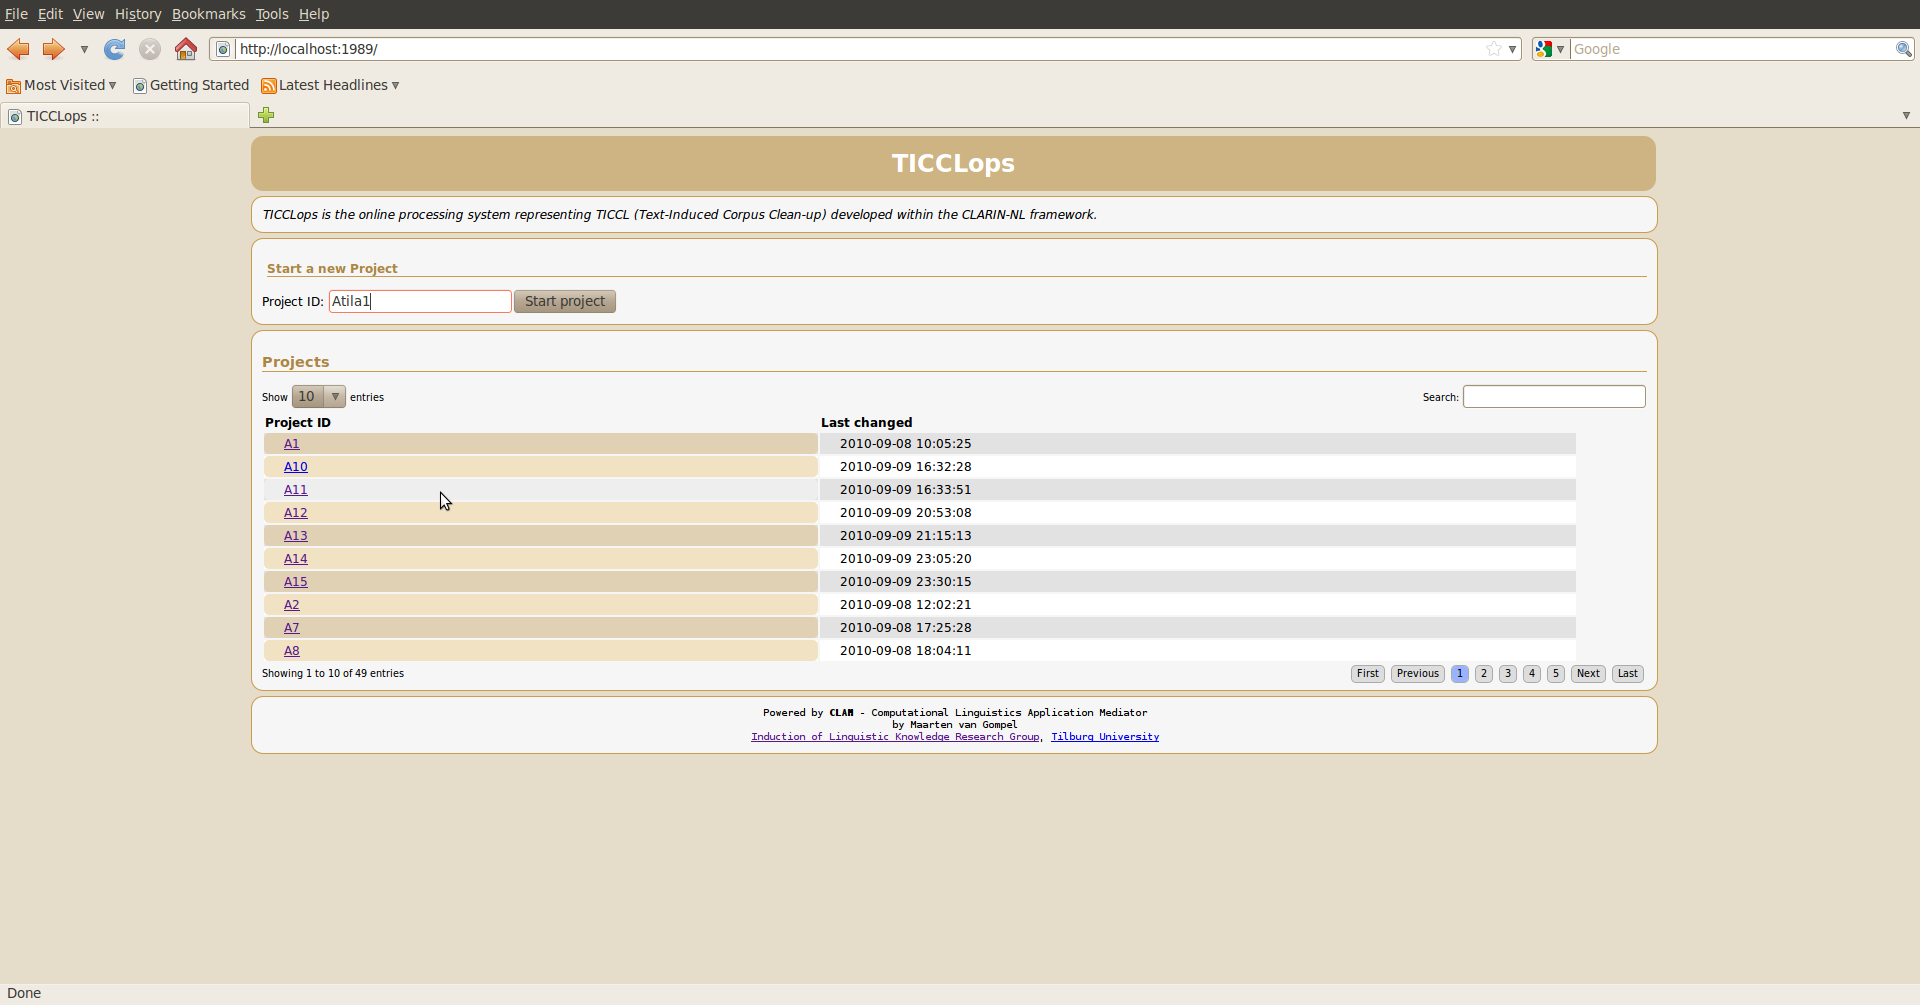
\includegraphics[width=130.0mm]{Screenshot-TICCLops.png}
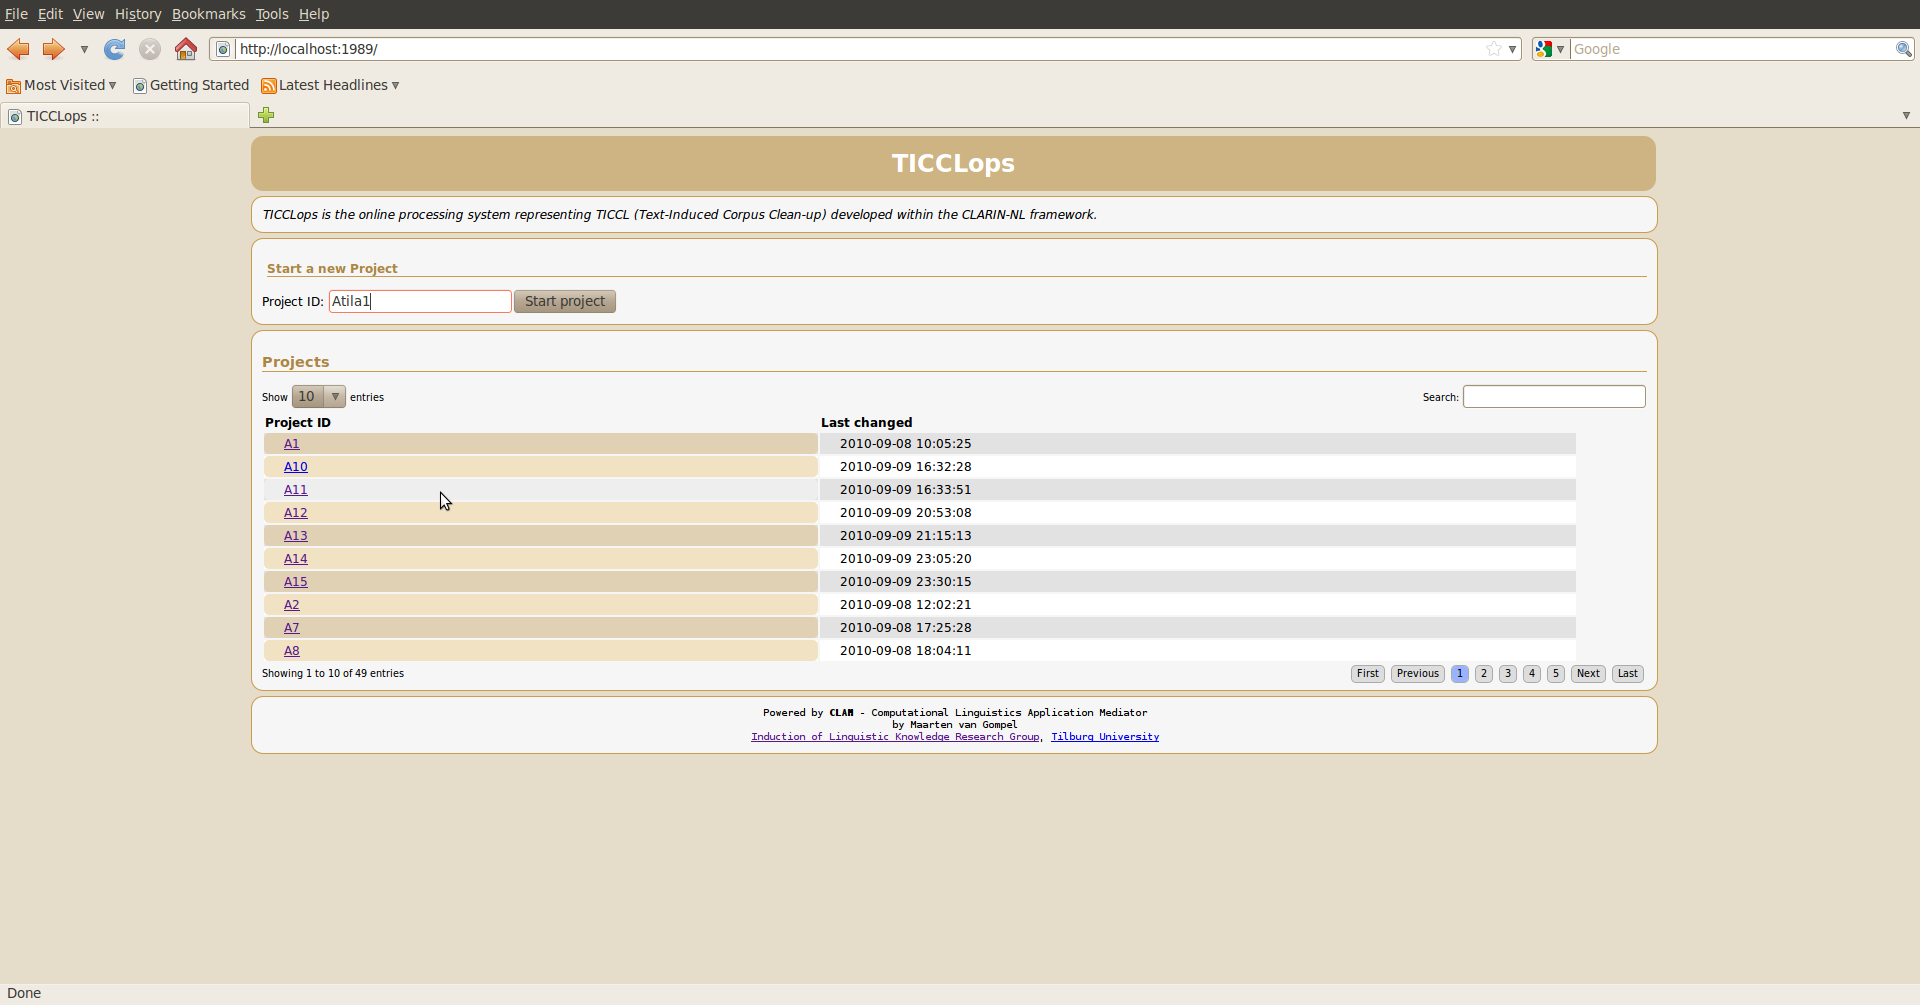
\includegraphics[scale=0.29,angle=90]{Screenshot-TICCLops.png}
\end{center}
\caption{TICCL project screen}
\label{projectscreen} 
\end{figure}

The first thing to do when working with TICCL is to make a project. If you have already specified a project before, you can also choose this project from a list. If you want to start a new project, type the name in the field Project ID and click {\it Start project}. In order to choose an existing project, you can click on its name in the list of Project IDs.

To run the demonstrator, you should create a new project, and choose a name you consider suitable.

\section{Step 2: Specify input}

Figure~\ref{inputscreen} shows the TICCLops screen for input selection.

\begin{figure}[h]
\begin{center}
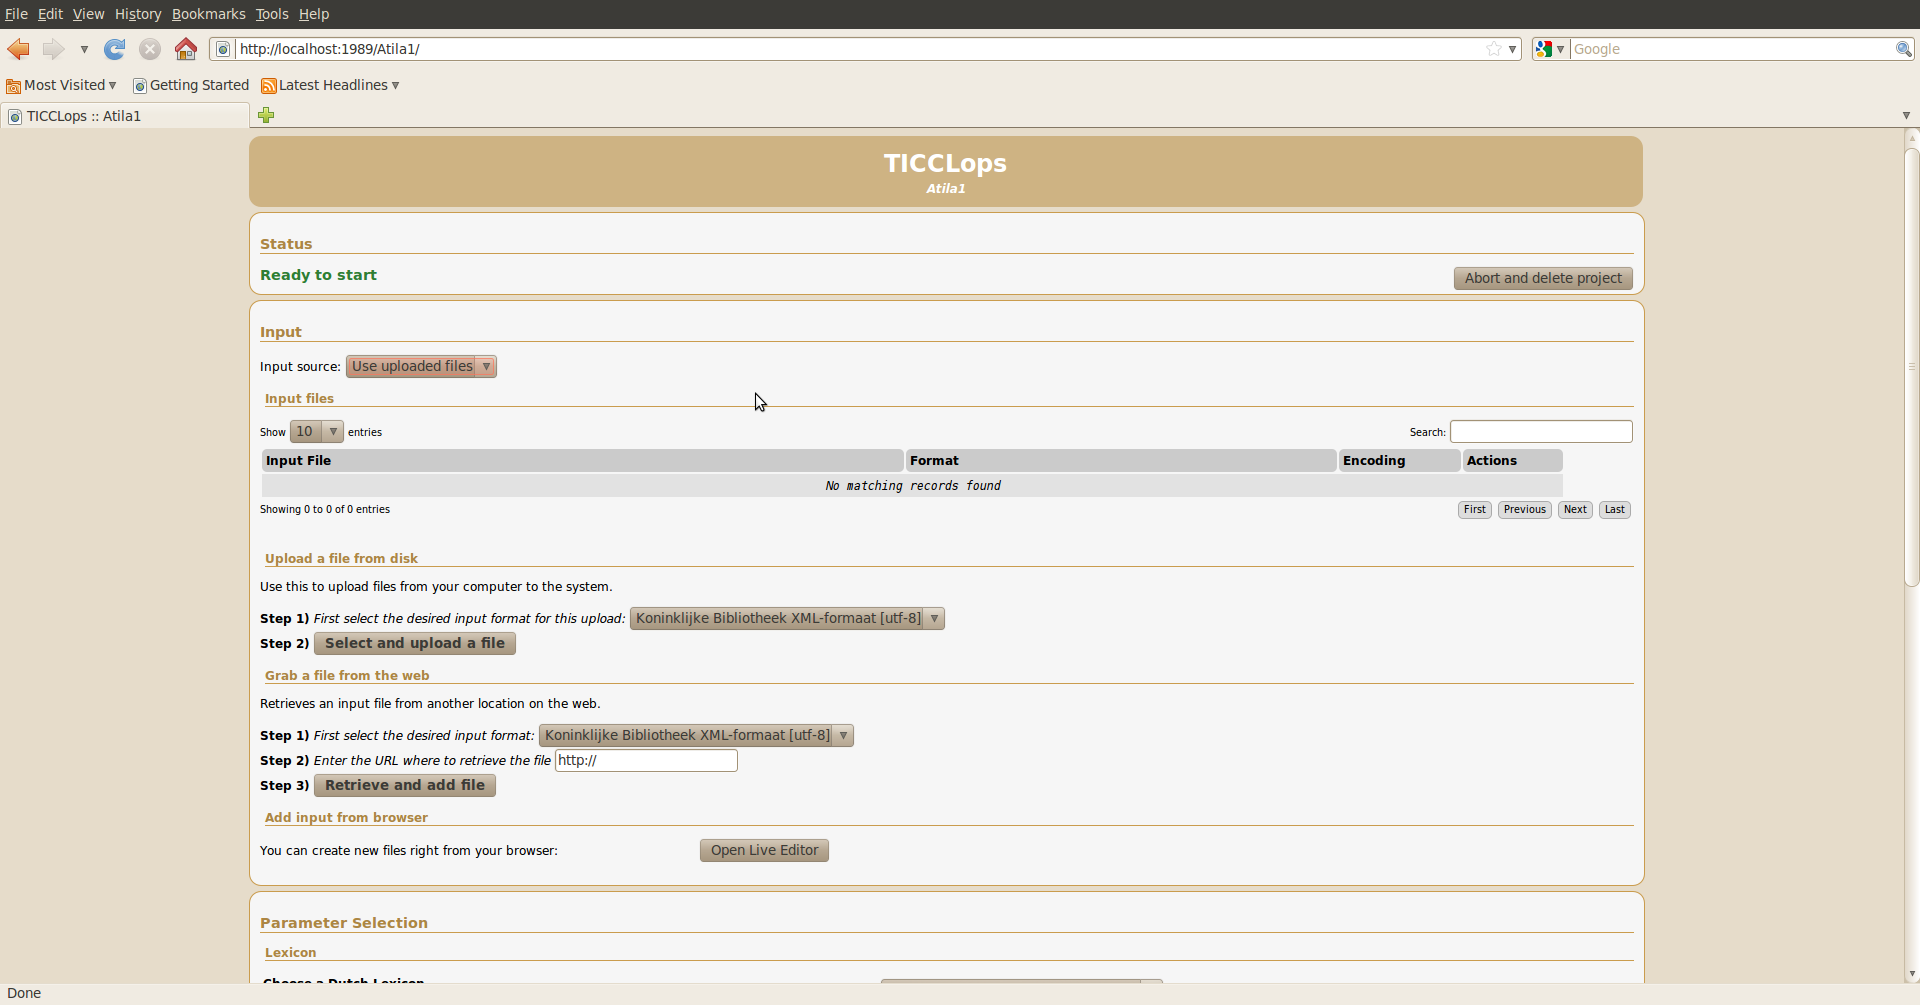
\includegraphics[scale=0.29,angle=90]{Screenshot-TICCLops1a.png}
\end{center}
\caption{TICCL input specification}
\label{inputscreen} 
\end{figure}

A choice has to be made what input source TICCL should use. The next step is to specify the corpus files you want TICCL to process. There are several options:

Pre-installed corpora may be available. The TICCLops demonstrator comes with the Martinet book as such a pre-installed corpus. You may choose to explore the system by way of this. This is done by selecting the first input button {\it Use uploaded files}. A dropdown box will show the available pre-installed corpora. Choose {\it OCR} to work with the demonstrator book.

Upload a file from disk

First choose the correct input format of the file that will be uploaded. This is done with the dropdown list. The choices available in this demo are:

\begin{itemize}
\item Koninklijke Bibliotheek XML-formaat [utf-8]
\item Plain Text Format (not tokenized) [utf-8]
\end{itemize}

Next, click button {\it Select and upload a file}, to choose the file from your file system.

Grab a file from the web

When choosing to grab a file that is available on the internet, the correct format must also be specified, using the dropdown list. The available formats are the same as for the previous choice. Next, the URL of the file to be retrieved must be entered, and then click button {\it Retrieve and add file}.

Add input from browser

It is also possible to create an input file using an editor. In order to do this, click button {\it Open Live Editor} and an editor will be started, as shown in Figure 3. Now text can be typed or copied into the input field, and saved under a chosen name. Also here the format of the text should be specified using the dropdown list.

Press {\it Add to input files} to save the document as an input file, or press {\it Cancel} to leave this screen without saving.

%For demonstration purposes choose the file Martinet.txt to upload (TODO?) and choose Plain Text Format as the input format.

Figure~\ref{editorscreen} shows the TICCLops editor to create a new file.

\begin{figure}[h]
\begin{center}
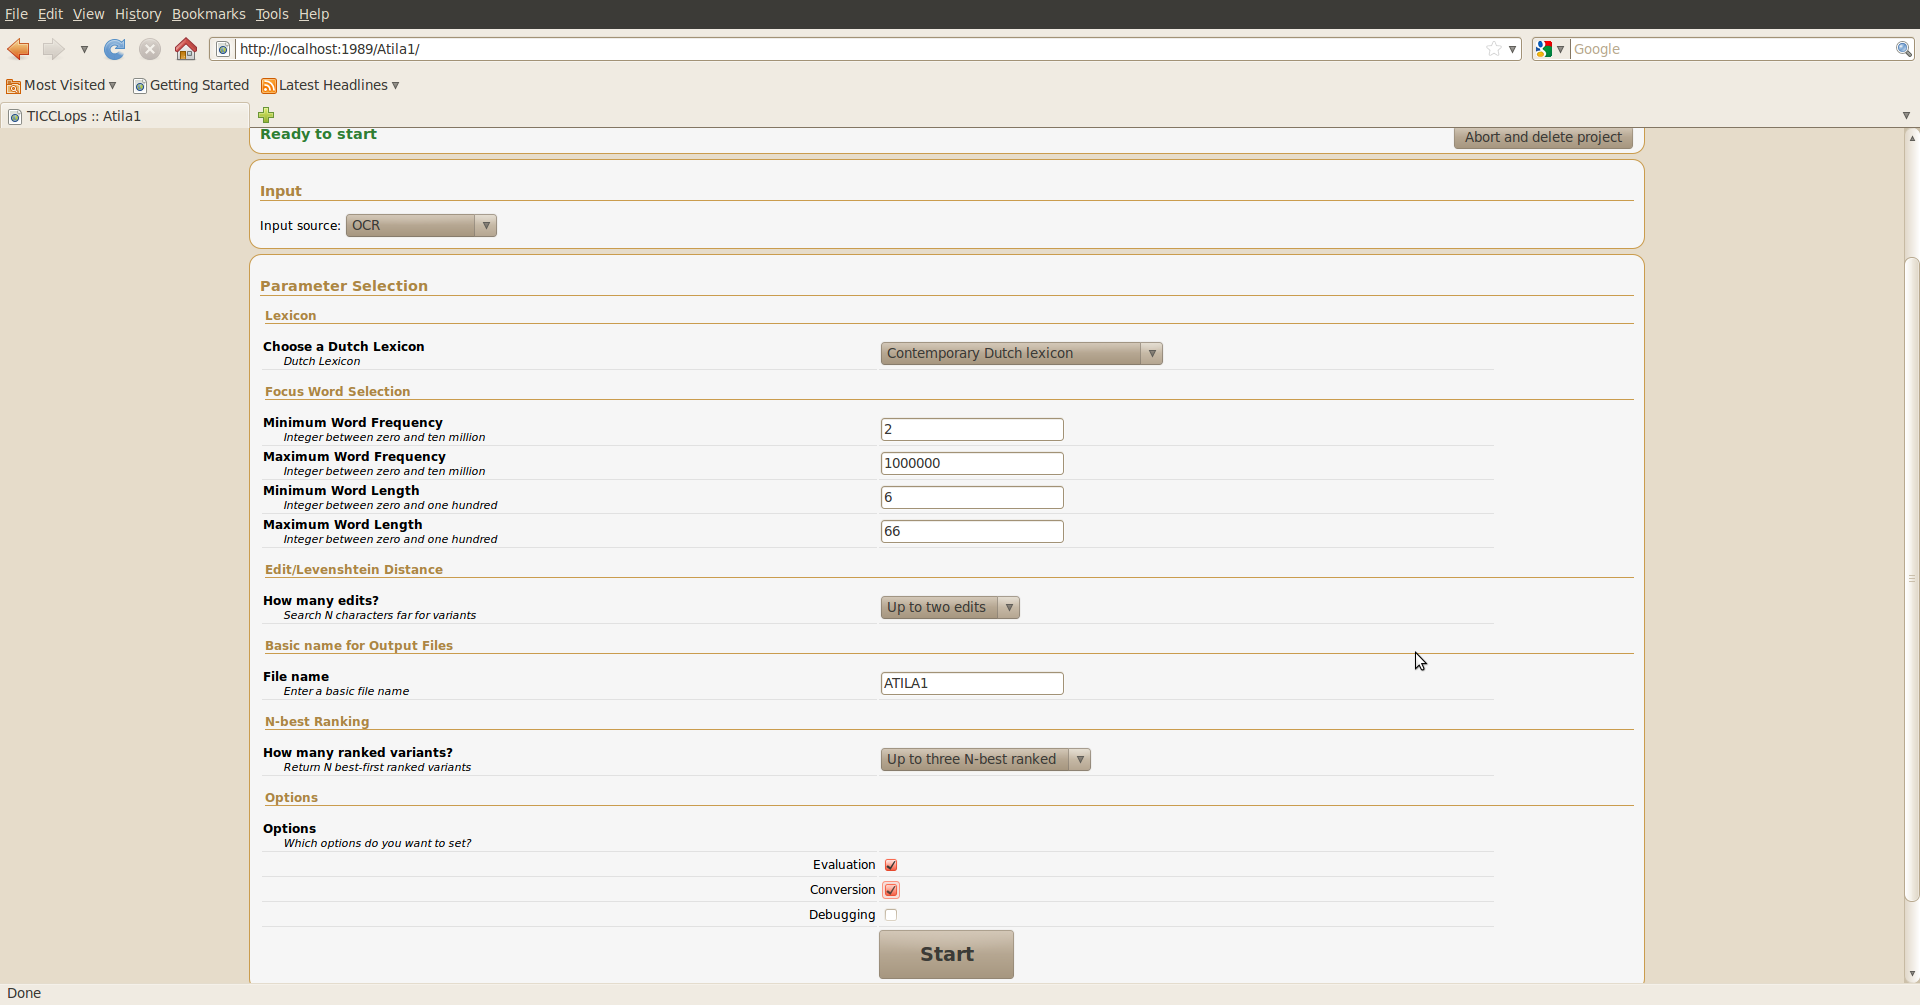
\includegraphics[scale=0.29,angle=90]{Screenshot-TICCLops2.png}
\end{center}
\caption{TICCL input editor}
\label{editorscreen} 
\end{figure}

\section{Step 3: Parameter selection}

Figure~\ref{parameterscreen} shows the TICCLops screen for parameter selection.

\begin{figure}[h]
\begin{center}
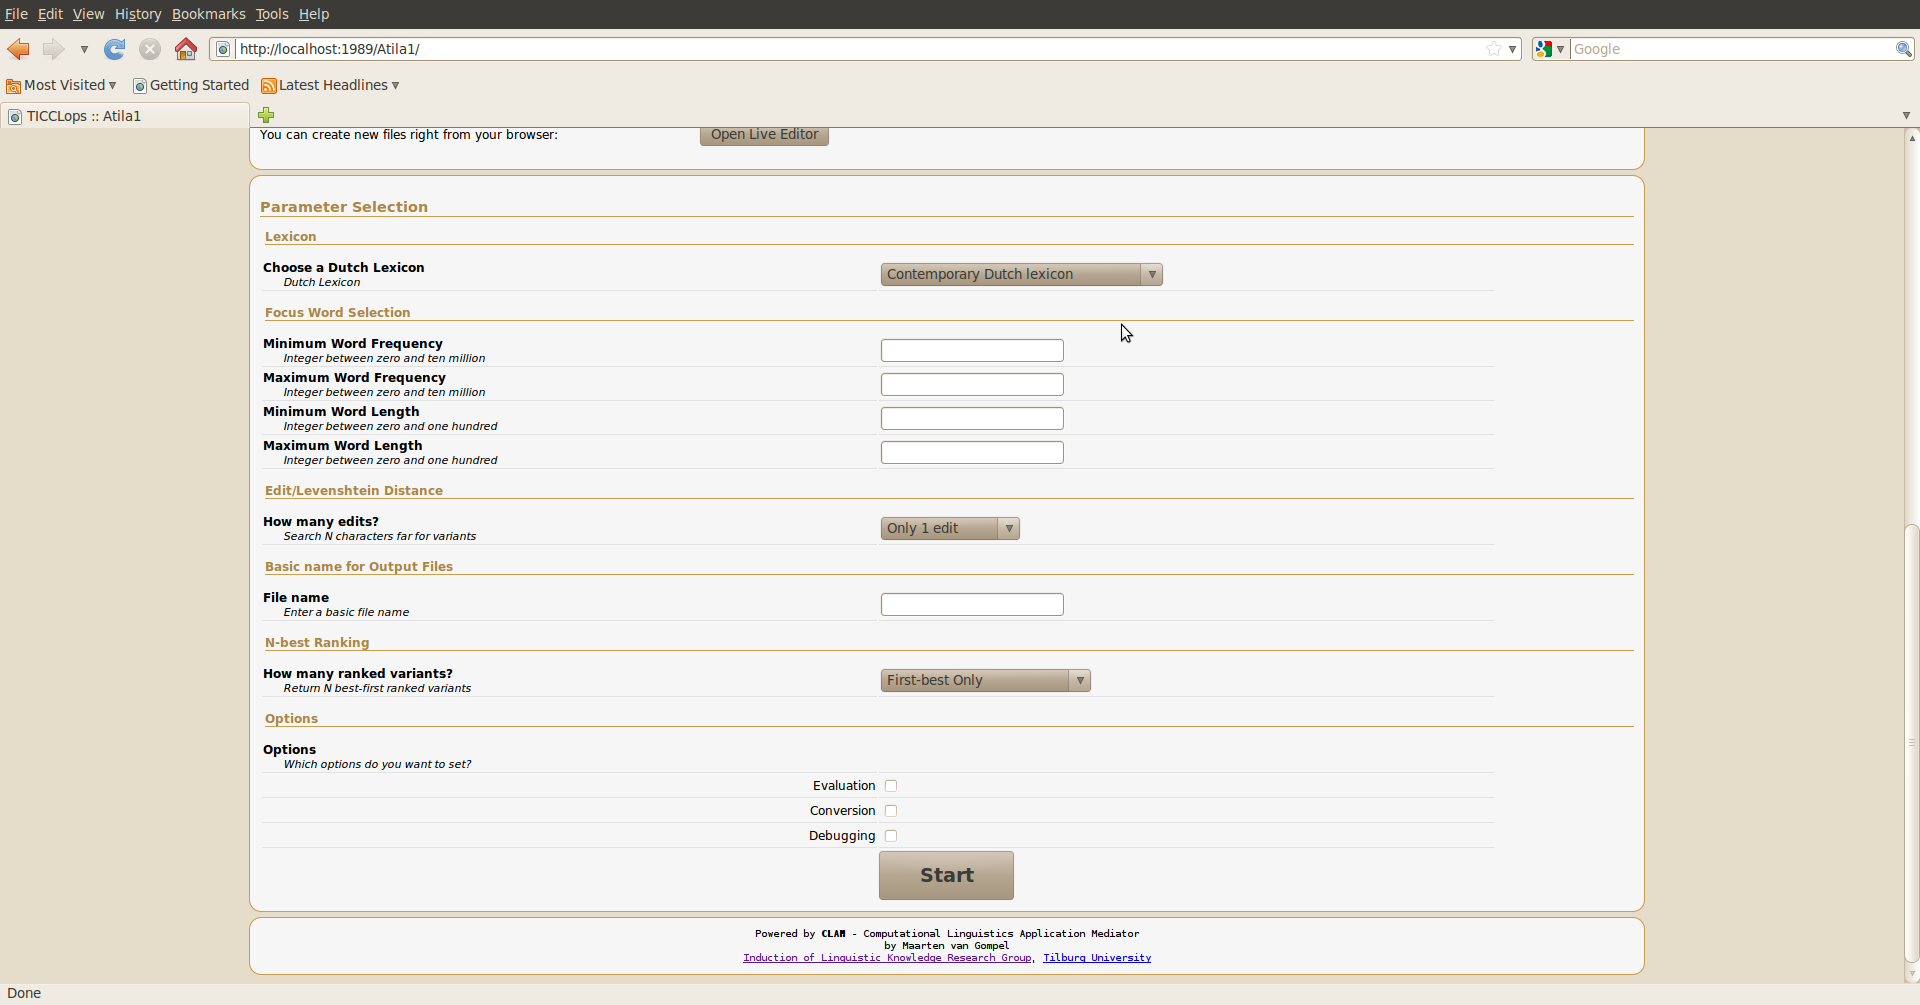
\includegraphics[scale=0.29,angle=90]{Screenshot-TICCLops1b.png}
\end{center}
\caption{TICCL input specification}
\label{parameterscreen} 
\end{figure}

Next, parameters have to be selected, to run TICCL with the desired options.

Choose a lexicon to use, from the dropdown list. The options available in this demo are:

\begin{itemize}
\item Contemporary Dutch lexicon
\item Historical/contemporary Dutch lexicon
\item No validated Dutch lexicon
\end{itemize}

TICCL can run very well without a supporting dictionary because the vocabulary present in the corpus plays an integral role in the variant retrieval process. This makes TICCL far less domain sensitive than most other approaches to spelling correction. In fact, experiments have shown that the larger the corpus TICCL is asked to process, the more reliable the observed word frequency statistics are and the better the results.

The selection criteria for the focus word need to be chosen. The word frequency minimum and maximum can have a value between 0 and 10 million, and the minimum and maximum length of the focus word can be set anywhere from 0 to 100.

Selection 1: only words appearing on a certain list are to be selected. Words on the list that do not appear in the corpus are not used as focus words. The list should have extension .lst.

Selection 2: specify the limits in frequency and word length not in relation to the corpus. Minimum and maximum frequency can be specified, and minimum and maximum word length in bytes/iso-8859-1 characters. Because the maximum frequency is not known before running TICCL, it can be useful to set this at a high value. It is not advisable to run TICCL on very short words, i.e. shorter than 5 characters, on badly OCR-ed corpora. When going for shorter words, the LD-limit must be conservative.\\

Example: 1000000-2-5-50 selects all words whose frequency lies between 2 and one million occurrences (including 2), with a word length between 5 and 50 (including 5 and 50).\\

Another parameter that needs to be set is the maximum edit distance (Levenshtein distance) between variants. This can be 1, 2 or 3. This parameter defines the scope of the search for lexical variants within the corpus.

Next, you need to specify a name that will be the prefix for all output files.

With N-best ranking the number of output canonical variants of a corpus word is limited. A choice can be made from 1, 2, 3, 5, 10 or 20 N-best ranked. In all cases the variants output are ranked, best candidate first.

Finally there are some options, that can be switched on with the checkboxes. These options are off by default.

\begin{itemize}
\item Conversion: Tick this box when your input date is in UTF-8 encoding.
\item Text Correction: when this box is checked your input files will be rewritten and the canonical forms for variants within your corpus will be added. The original word form is not overwritten, but rather enriched with the number of n-best canonical forms requested earlier (if, indeed, so many were found).
\item Evaluation: This option only makes sense when indeed a gold standard for the corpus is available, as is the case for the TICCLops demonstrator. By checking this box, the output of TICCLops given its input parameter settings is compared with the expected outcome given the gold standard and scored on various levels. A full report of this can be found in the log file after processing has finished.
\end{itemize}

For demonstration purposes you might choose the following:

%\begin{itemize}
\begin{itemize}
\item lexicon: Historical-contemporary Dutch lexicon
\item word frequency: 1-250
\item word length: 6-100
\item maximum edit distance: 2
\item output file names prefix: as desired, preferably shorter than 25 characters
\item N-best ranking: Up to 3 N-best ranked
\item checkboxes Evaluation and Conversion are to be checked
\item check box Text Correction if you want the actual input files to be rewritten
\end{itemize}

Next, click {\it Start}.

\section{Step 4: Processing}

Figure~\ref{progressscreen} shows the TICCLops screen for monitoring processing progress .

\begin{figure}[h]
\begin{center}
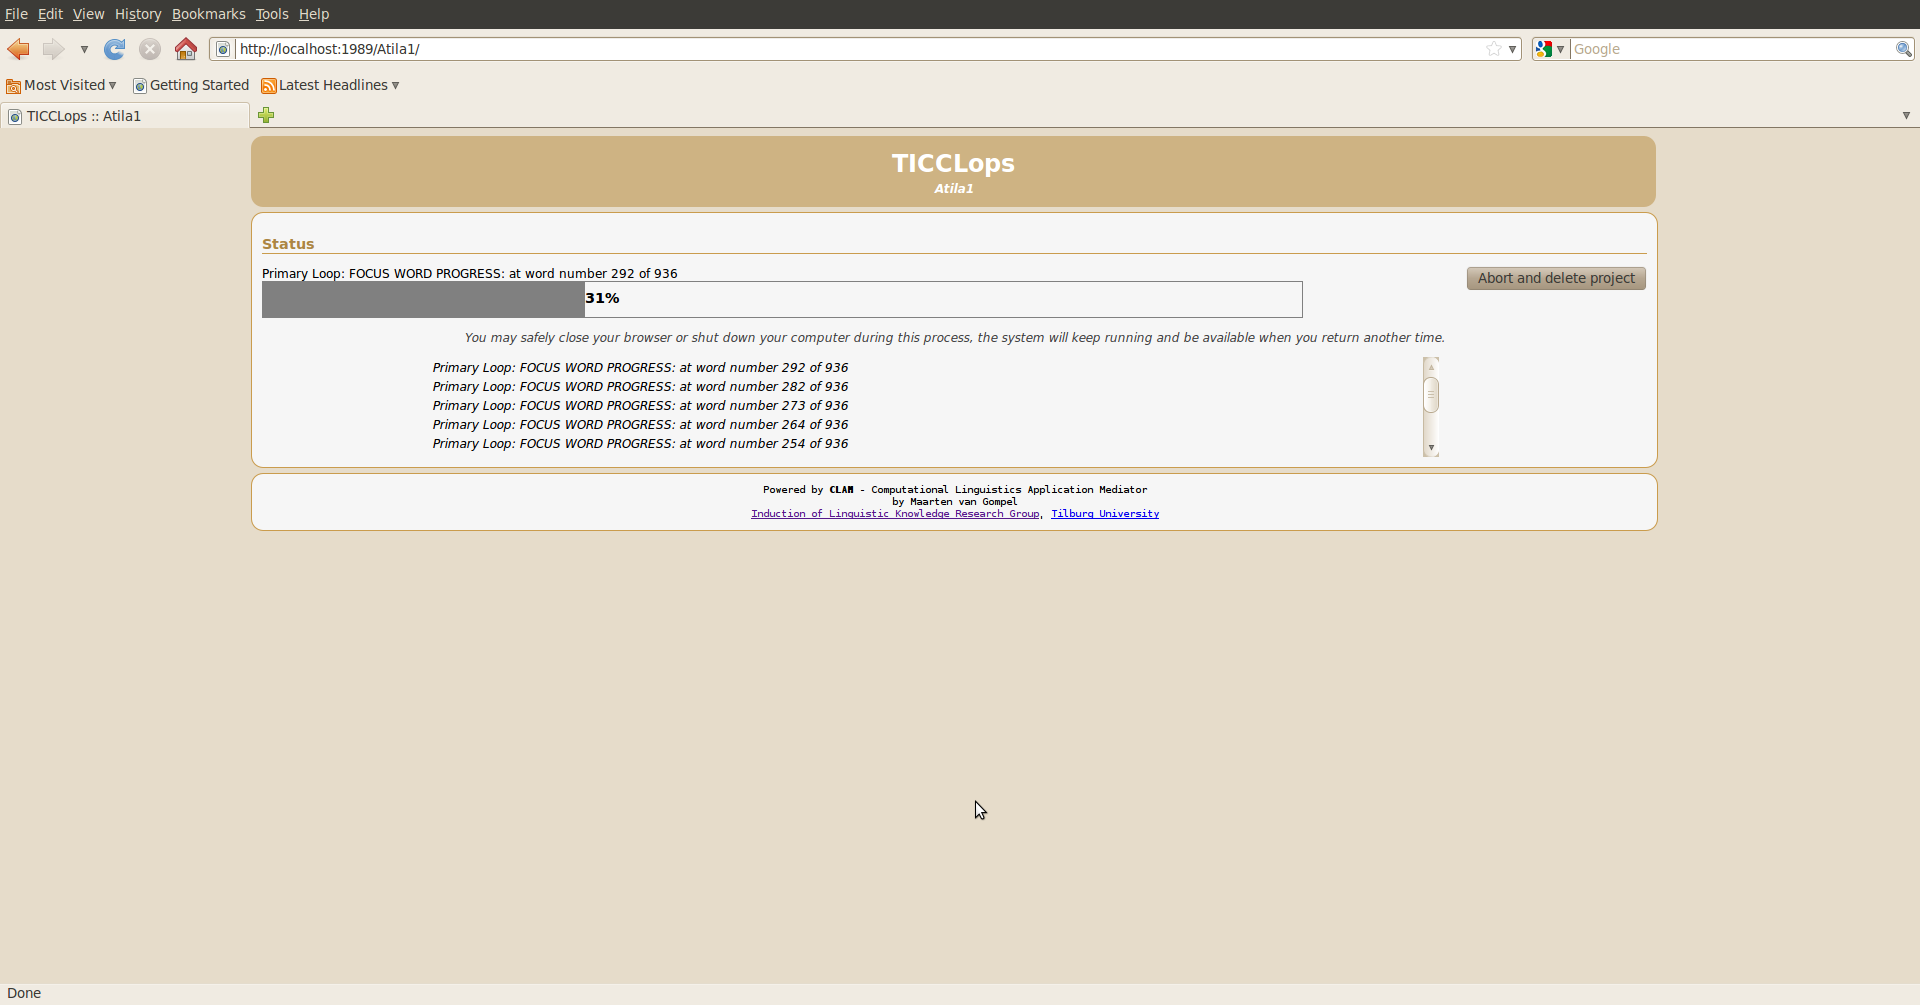
\includegraphics[scale=0.29,angle=90]{Screenshot-TICCLops3.png}
\end{center}
\caption{TICCL processing progress}
\label{progressscreen} 
\end{figure}

While TICCL is running, the status of the process is shown on the screen, and is regularly updated. It is not necessary to leave the browser open while the process is running. You can close the window and come back later. If you want to reopen the process you were running, start TICCL again and choose the project you started from the list.

It is also possible to stop TICCL running, by clicking {\it Abort and delete project}. This stops the process, and deletes all the uploaded input files and possibly generated output files, and the project.

\section{Step 5: Output}

Figure~\ref{outputscreen} shows the TICCLops screen for output viewing or downloading.

\begin{figure}[h]
\begin{center}
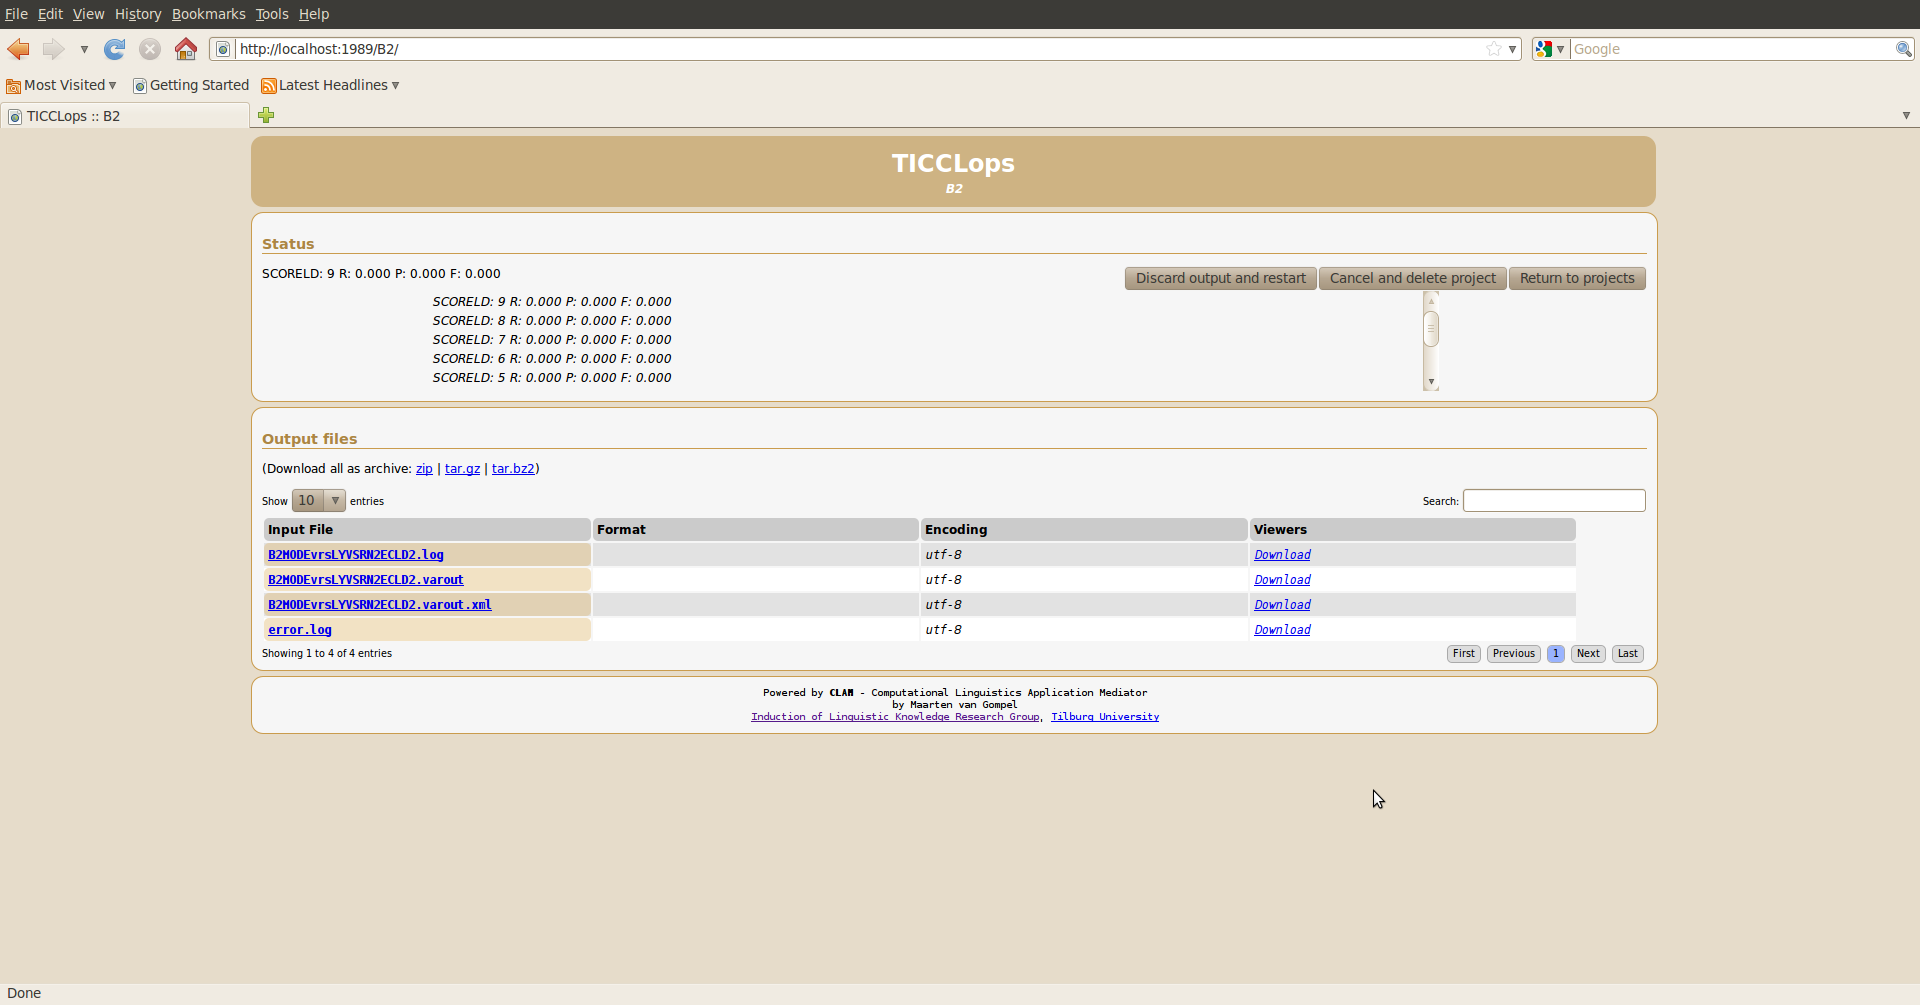
\includegraphics[scale=0.29,angle=90]{Screenshot-TICCLops5.png}
\end{center}
\caption{TICCL output viewing or downloading}
\label{outputscreen} 
\end{figure}

After TICCL processing is done, the output files are shown. They can be viewed separately by clicking on them, and they can be downloaded bundled together as an archive. Several archive formats are possible: zip, tar.gz and tar.bz2. To download the files in compressed format, click the format of choice.
Clicking {\it Discard output and restart} deletes all the uploaded input files and possibly generated output files, and restarts the project.
Clicking {\it Cancel and delete project} deletes all the uploaded input files and possibly generated output files, and the project itself.
If you want to temporarily leave your project, you can close your browser, and open your project again at a later time.

\chapter{TICCLops Output}

%TICCL is always run with a corpus as input. This corpus can consist of one or more text files. Depending on the parameter settings, the words in the corpus will be listed together with their canonical form.

TICCL gives a list as output, consisting of word pairs where the left hand word is the canonical form, and the right-hand word is the normalized variant of the word, as found in the corpus. This variant can differ from the canonical form because of a typesetting error, spelling or typographical error, OCR error, historical spelling difference, or a combination of these.

%\section{Input files}

%required:?corpus?lexicon *?
%TICCL is shipped with ready-made versions of the input files marked with *. Custom files can also be used.

\section{Output files}

Detailed output (.varout.xml)?
Contains the same information as the short output, but in an XML-format. Also the surface forms of the normalized variants are added.

Example: 


Log file (.log)?
contains information about which corpus files were processed, along with the processing time per file, the number of word forms (types) and the total number of words (tokens) found in the corpus, and the type/token ratio. ?If TICCL was run with an evaluation file, the results of the evaluation are also in the log file. The log file ends with the total time run.

%Optional output

%Simple output file (.varout)?%When the S-switch is specified, simple output for varout.xml is created like this. Each line consists of the normalized variant, corpus frequency of that variant, focus word, corpus frequency of the focus word, Levenshtein distance between the two, and the surface forms in pseudo-XML. This XML-structure is necessary, because the surface forms may contain any character, including the #-delimiter. This delimiter cannot appear in normalized forms or focus words.
%noemenswaanl#1#noemenswaar#3#2#<InCorpus>noemenswaanl</InCorpus>
%noemenswaardigen#1#noemenswaardige#8#1#<InCorpus>noemenswaardigen</InCorpus>
%noemenswaardigen#1#noemenswaardig#5#2#<InCorpus>noemenswaardigen</InCorpus>

Error log file (error.log)?When something goes wrong during TICCL�s processing it will be logged in this file.



%\section{}

%\section{Architecture}

%In Figure~\ref{} 

%\begin{figure}[h]
%\begin{center}
%\includegraphics[width=130.0mm]{}
%\end{center}
%\caption{The CLAM Architecture}
%\label{} 
%\end{figure}

%A CLAM webservice needs the following three components from the service developer:

%\begin{enumerate}
%\item A service configuration file
%\item A wrapper script for your NLP application
%\item An NLP application
%\end{enumerate}


%\begin{devnotes}
%The CLAM Frontend, the green outer layer in Figure \ref{fig:arch} does not exist yet.
%\end{devnotes}


%\section{}
%\label{}

%All parameters can take the following extra named arguments:

%\begin{itemize}
%\item \textbf{\texttt{default}} - Set a default value.
%\item \textbf{\texttt{required}} - Set to \texttt{True} to make this parameter required rather than optional.
%\item \textbf{\texttt{require}} - Set this to a list of parameter IDs. If this parameter is set, so must all others in this list.
%\item \textbf{\texttt{forbid}} - Set this to a list of parameter IDs. If this parameter is set, none of the others in the list may be set.
%\item \textbf{\texttt{allowusers}} - Allow only the specified lists of usernames to see and set this parameter. If unset, all users will have access. You can decide whether to use this option or \texttt{denyusers}, or to allow access for all.
%\item \textbf{\texttt{denyusers}} - Disallow the specified lists of usernames to see and set this parameter. If unset, no users are blocked from having access. You can decide whether to use this option or \texttt{allowusers}, or to allow access for all.
%\end{itemize}

\bibliographystyle{spbasic}
\bibliography{TicclopsManual.bib}

\end{document}
